\chapter{Grundlagen}

In dieser Arbeit werden grundlegende Kenntnisse in der Entwicklung von Betriebssystem und der Verwendung eines Debuggers vorausgesetzt. Bestimmte Begriffe und Konzepte werden daher nachfolgend ohne ausführliche Erklärung verwendet. Die wichtigsten Grundlagen zum Verständnis dieser Arbeit werden in diesem Kapitel jedoch kurz erläutert.

\section{Rust}
Rust kombiniert die Möglichkeit, hardwarenahe Details, wie Speicherzugriffe, selber zu kontrollieren, was normalerweise mit viel Aufwand verbunden ist, mit einer hohen Nutzerfreundlichkeit. Es wird viel Wert sowohl auf Geschwindigkeit, als auch auf Stabilität gelegt. Der Compiler schließt viele Bugs bereits zur Compilezeit aus, was späteres Testen und Suchen verringert \cite{rust-lang}. 

\section{D3OS}
Das D3OS (Distributed Data-Driven OS) ist ein in Rust entwickeltes, verteiltes Betriebssystem, das speziell für moderne Rechenzentrenhardware und skalierbare, datenintensive Anwendungen entworfen wurde. Es setzt auf verteilte Ressourcenverwaltung, einen Shared-nothing Microkernel, sowie schnelle Netzwerktechnologien \cite{d3os}. Der Quellcode zu D3OS ist auf GitHub zu finden und wird von der Abteilung für Betriebssysteme der HHU betreut und entwickelt \cite{d3os-repo}. \\
Bei einem Microkernel handelt es sich um eine Architektur, bei welcher der Kernel nur grundlegende Dienste, wie zum Beispiel Allokation von physischem Speicher und Scheduling übernimmt, während andere Komponenten, wie das Dateisystem, modular als Server im User-Space realisiert werden. Dadurch sind Microkernels zwar stabiler und flexibler, da ein fehlerhafter Dienst nicht direkt den Kernel beeinflusst, aber auch langsamer als monolithische Kernels, da mehr Prozesse miteinander kommunizieren müssen und mehr Kontextwechsel stattfinden \cite{microkernel}.

\section{GDB}
Bei GDB handelt es sich um einen weit verbreiteten Open-Source Debugger. GDB unterstützt viele verschiedene Sprachen, darunter auch das in D3OS verwendete Rust und kann sowohl lokal, als auch remote auf einem anderen Zielsystem verwendet werden \cite{gdb}. 

\section{Remote Debugging}
Wie bereits erwähnt bietet GDB die Möglichkeit auf einem Hostrechner ausgeführt zu werden und dabei ein anderes Zielsystem zu debuggen. Das wird über das GDB RSP (Remote Serial Protocol) und einen sogenannten Debugging Stub realisiert. Der Stub läuft auf dem Zielsystem und bildet die Schnittstelle zwischen GDB und dem zu untersuchendem System. Dadurch kann GDB das Zielsystem steuern und dessen Zustand analysieren, ohne dass der Debugger vollständig implementiert werden muss. Das Zielsystem muss besondere Subroutinen implementieren um mit GDB zu kommunizieren und die empfangenen Befehle auszuführen \cite{gdb}. In dieser Arbeit wird die Kommunikation über den seriellen Port und die Auswertung der Pakete durch die Rust Crate \texttt{gdbstub} umgesetzt. Die Crate implementiert das GDB RSP und bietet Schnittstellen an, in denen man das Verhalten des Zielsystems definieren muss \cite{gdbstub}. 

\section{Verwandte Projekte}
Der Autor der Crate verweist in der Dokumentation auf eine Sammlung beispielhafter Implementierungen. Die Beispiele bieten einen ersten Überblick über die Crate für verschiedene Anwendungsfällen und Architekturen \cite{gdbstub}. Außerdem gibt es eine Implementierung des GDB RSP ohne die Crate für hhuOS \cite{hhuos}.

\section{Umsetzung von GDB Befehlen über das Remote Serial Protocol}
Nicht jedem GDB Befehl ist auch ein entsprechendes Paket zugeordnet. Manche Befehle werden durch mehrere verschiedene Pakete von GDB zusammengesetzt. Durch den Befehl \texttt{set debug remote 1} zeigt GDB die geschickten und empfangenen Pakete nach jedem Befehl an \cite{gdb}. Im Folgenden wird die Funktionsweise der wichtigsten Befehle erläutert.

\subsection{Lesen \& Schreiben von Speicher}
Um Variablen zu lesen und zu schreiben nutzt GDB beim remote Debugging eine Kombination aus den Register- und Adressfunktionen. Wenn man zum Beispiel in einer Funktion \texttt{foo} einen Breakpoint trifft und an GDB meldet, dann holt sich GDB zusätzlich noch den Registerzustand und liest einen Teil vom Stack aus. Wenn man dann eine lokale Variable \texttt{bar} auslesen möchte, berechnet GDB die Adresse als Kombination aus dem Wert vom Base Pointer und einem Offset. Danach kann GDB den Wert aus dem Stackbereich direkt auslesen, ohne weitere Pakete an den Stub zu schicken.

\subsection{Continue von einem Breakpoint}
Bei Software Breakpoints auf der \texttt{x86-64} Architektur wird das erste Byte der Instruktion an der Stelle des Breakpoints durch die Breakpointinstruktion \texttt{0xCC} ersetzt. Wird diese Instruktion ausgeführt, löst die CPU eine Breakpoint Exception aus. Dabei zeigt der Instruction Pointer auf die Adresse hinter der Breakpointinstruktion. Damit das Programm nach dem Stopp korrekt fortgesetzt werden kann, sind folgende Schritte nötig \cite{intel-sdm}:

\begin{enumerate}[]
\item Instruction Pointer um eins reduzieren, weil er auf die Instruktion nach dem Breakpoint zeigt
\item Breakpoint durch Originalbyte ersetzen
\item Trap Flag setzen, damit nach einer Instruktion wieder eine Exception ausgelöst wird
\item Instruktion ausführen
\item Breakpoint wieder zurückschreiben
\end{enumerate}

 GDB übernimmt aber Teile der Logik, sodass nicht alles im Breakpoint-Handler gemacht werden muss. Wenn der Stub meldet, dass ein Breakpoint getroffen wurde, liest GDB Register und Speicher aus und entfernt dann den Breakpoint. Das Originalbyte wird also durch die \texttt{remove\_sw\_breakpoint} Funktion des Stubs zurückgeschrieben. Wenn man jetzt vom Breakpoint aus fortfahren will, schickt GDB typischerweise zuerst einen Step-Befehl, es soll also nur die nächste Instruktion ausgeführt und dann eine Debug Exception ausgelöst werden. Sobald GDB wieder die Kontrolle nach dem Step bekommt, setzt es den Breakpoint erneut ein und schickt dann entweder einen Continue-Befehl, wenn der Nutzer davor selber einen Continue-Befehl eingegeben hat oder wartet auf weitere Anweisungen. Der Breakpoint-Handler muss also noch den Instruction Pointer reduzieren, während der Rest der Logik durch verschiedene GDB Pakete zusammengesetzt und die entsprechenden Funktionen des Stubs ausgeführt wird. Die Unterschiede zwischen dem Handler im Stub und einem normalen Handler kann man auch in Grafik \ref{breakpoint_grafik} sehen.
 
 \begin{figure}[h]
  \centering
  \begin{subfigure}[b]{0.4\textwidth}
  \centering
    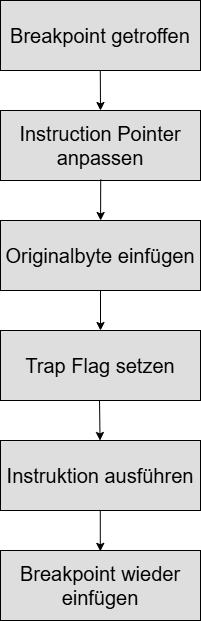
\includegraphics[width=\linewidth,height=0.4\textheight,keepaspectratio]{img/BPAblauf.drawio}
    \caption{Breakpoint Behandlung ohne Stub}
    \label{grafik_2}
  \end{subfigure}
  \begin{subfigure}[b]{0.45\textwidth}
  \centering
    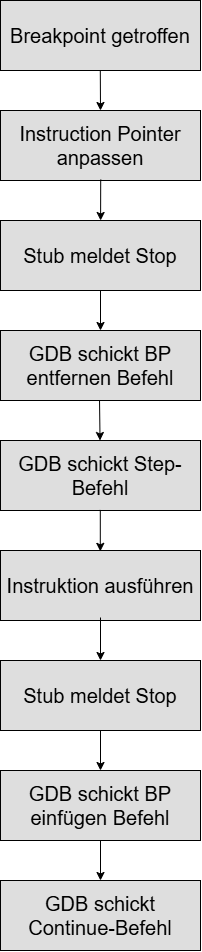
\includegraphics[width=\linewidth,height=0.4\textheight,keepaspectratio]{img/BPAblaufGDB.drawio}
    \caption{Breakpoint Behandlung mit Stub}
    \label{grafik_3}
  \end{subfigure}
  \caption{Unterschiede Breakpoint Behandlung}
  \label{breakpoint_grafik}
\end{figure}

\subsection{Step Into}
Durch den Befehl \texttt{step} oder \texttt{s}, wird das Zielprogramm ausgeführt, bis es die nächste Zeile im Quellcode erreicht. Sollten dafür mehrere Instruktionen ausgeführt werden müssen, schickt GDB auch mehrere \texttt{step} Befehle und liest den Speicher aus, bis es erkennt, dass die nächste Zeile erreicht wurde. Dabei werden Funktionsaufrufe nicht direkt ausgeführt, sondern GDB schreitet in die Funktion. Das wird über temporäre Software Breakpoints realisiert. Wenn GDB den Funktionsaufruf sieht, setzt es einen Software Breakpoint an der Adresse der aufgerufenen Funktion und lässt das Programm weiter laufen, bis der Breakpoint erreicht wird. 

\subsection{Step Over}
Mit dem Befehl \texttt{next}, beziehungsweise \texttt{n}, wird das Zielprogramm ebenfalls bis zur nächsten Zeile im Quellcode ausgeführt. Dabei werden Funktionen aber nicht betreten, sondern direkt vollständig ausgeführt. Dazu setzt GDB einen Software Breakpoint auf die Zeile nach dem Funktionsaufruf. Danach wird das Zielprogramm weiter ausgeführt bis es den Breakpoint erreicht. Es wird also alles bis zur nächsten Zeile in der aktuellen Funktion ausgeführt.